\section{Method}\label{sec:yourmethod}
We present our two different approaches to parallelize the algorithm and their major optimizations. Our implementations use MPI (``Message Passing Interface''). We also discuss a vectorization optimization that can be applied to both versions. Our source code and test cases are publicly available \cite{our_source}.


% Now comes the ``beef'' of the report, where you explain what you did. 
% Again, organize it in paragraphs with titles. As in every section
% you start with a very brief overview of the section.
% In this section, structure is very important so one can follow the technical content.
% Mention and cite any external resources that you used including libraries or other code.

\mypar{Row-wise algorithm}
The design of our algorithm is intentionally simple. We divide each row of our pyramid-shaped DP table into evenly spaced contiguous segments and assign exactly one to each worker. As the number of cells in each row is increased by one we increase the size of a segment by one. To ensure a balanced workload we increase each segment size in a round robin fashion.

Each worker calculates the cells in its segment from left to right. But in order to calculate the leftmost element the worker may depend on the rightmost element of the previous row from the left neighboring worker. Thus a worker has to wait for the neighboring worker to complete its segment in the previous row before the worker can start the next row. This can lead to an imbalance. In order to overcome this issue we prioritize the leftmost and rightmost elements and calculate them first and send them right away before calculating any other elements. This ensures that the waiting time is minimal.
    
The number of messages sent in each row is constant in the number of workers (up to two receives and one send per worker) independent of the size of the rows. This means that with a small work size per worker we get a significant communication overhead. We solve this by first increasing the segment of a worker until it reaches a certain threshold before assigning any work to the next worker. In experiments we found that a threshold of $200$ cells works well.

We can calculate the edit script in a similar fashion as a sequential algorithm would. But due to the quadratic memory consumption we did not benchmark this.

\mypar{Dynamic priority algorithm}
In our row-wise algorithm a worker will not calculate any elements of the next row until it receives all required elements of the previous row. This blocking wait is usually not necessary - it is possible to calculate some elements of the next rows without waiting for other workers. We designed the dynamic priority algorithm to always perform some calculation instead of a blocking wait if possible. Additionally, the algorithm prioritizes calculations that will be sent to other workers, so that they are quickly unblocked.

\begin{figure}[hbt]\centering
  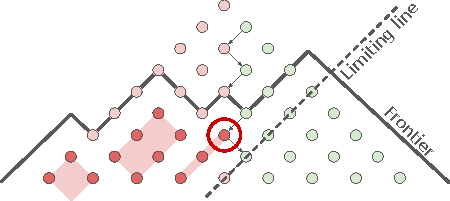
\includegraphics[width=0.85\linewidth]{images/dphpc-dynamic-priority-diagram.pdf}
  \caption{Visualization of the internal state of the dynamic priority algorithm. The circles are cells in the DP table (colored by worker). There are two workers (red and green). The state is from the perspective of the red worker. The arrows represent (past or future) sends and receives. Every cell on or above the \emph{frontier} is known to have been calculated by some worker. Every cell on or below the \emph{limiting line} cannot be calculated by the red worker at the moment.}
  \label{priority_state}
\end{figure}

In order to perform calculations whenever possible, it is necessary to determine which calculations are possible in a given state. Figure \ref{priority_state} shows the internal state that our algorithm keeps for this purpose. Every cell on the solid jagged line (\emph{frontier}) has been calculated by some worker, and every cell on or below the dotted line (\emph{limiting line}) can not be calculated at the moment. This means that all cells below the frontier and above the limiting line can be calculated without receiving any further messages from other workers. The frontier and the limiting lines fully determine the currently possible calculations (darker red).

The shape of the frontier is a direct consequence of the dependencies in our DP table. Before a DP cell can be calculated, the cells above it (left and right) must be calculated (see arrows in figure \ref{dp_table}). Because of transitivity, this means that all DP cells in the ``upside down pyramid'' ending in a cell must have been calculated before it. The frontier is the boundary of a union of such pyramids. Whenever a worker learns that a cell was calculated (because it calculated the value itself or received it from another worker) it extends its frontier by union with the pyramid ending in that cell.

Every worker has up to 2 limiting lines at any given time. These diagonal lines go through the next cell that the worker expects to receive. The worker shouldn't calculate any cells on or below a limiting line, since these cells will either be calculated by another worker (e.g. the cell that it expects to receive) or depend on values in such cells.

Once it is clear which cells are possible to calculate, it is necessary to choose a calculation order. One interesting case is outlined with a red circle in figure \ref{priority_state}. This cell has not been calculated yet, and another worker expects to receive its value. To prevent other workers from being blocked, such cells (and their dependencies) will be calculated before cells that do not result in a send. If there are no such cells to prioritize, cells near the middle of the DP pyramid are calculated first, since this order results in a frontier with few bends, which makes planning calculations faster.

\mypar{SIMD Optimization}
The amount of work needed per DP cell dynamically depends on the input, since the number of loop iterations in the while-loop is determined by the number of equal elements after a change. Therefore, the workload per worker might be imbalanced. %, especially for inputs with high similarity. 
To mitigate these imbalances and hence, reduce the time workers are waiting, we use x86's SIMD\footnote{``Single instruction stream, multiple data streams'' by Flynn's Taxonomy \cite{flynns_taxonomy}} vector extensions to compare multiple elements at once.

In many cases we need to compare only one value, because the first value is already unequal. In these cases we would not benefit from using SIMD instructions, they might even be more expensive. Therefore, we have a preliminary scalar check for inequality of the first element. Only if this check fails, we will use SIMD instructions.

%To force the compiler to use SIMD instructions we use the vector intrinsics from the \texttt{immintrin.h} %TODO: ref needed?) -> Intel intrinsics guide as footnote?
%header.
%If there are at least eight elements left in both input sequences, we will use the AVX\footnote{Advanced Vector Extensions and} instructions which operate on 8-way vectors of 32-bit integers. For the case, in which less than eight elements but at least four are left, we make use of SSE\footnote{Streaming SIMD Extensions are extensions to the x86 instruction set architecture} instructions once to compare 4-way vectors.

For the vectorized comparison we first load unaligned 8-way or 4-way vectors from both input sequences (the loads need to be unaligned, since we do not know the position in the vector in advance and we compare the input sequences at different offsets). Then we use a \texttt{cmpeq} intrinsic to compare the two vectors for equality. The result is then checked for an unequal element by using the negation of the \texttt{testc} intrinsic. If there is no inequality, the next vector will be checked. Otherwise, the exact location of the inequality is determined by a scalar loop over the last up to eight elements using the same loop as in the original algorithm.